\documentclass{standalone}
\usepackage{tikz}
\usetikzlibrary{patterns, positioning}
\usepackage[sfdefault]{ClearSans} %% option 'sfdefault' activates Clear Sans as the default text font
\usepackage[T1]{fontenc}

\begin{document}
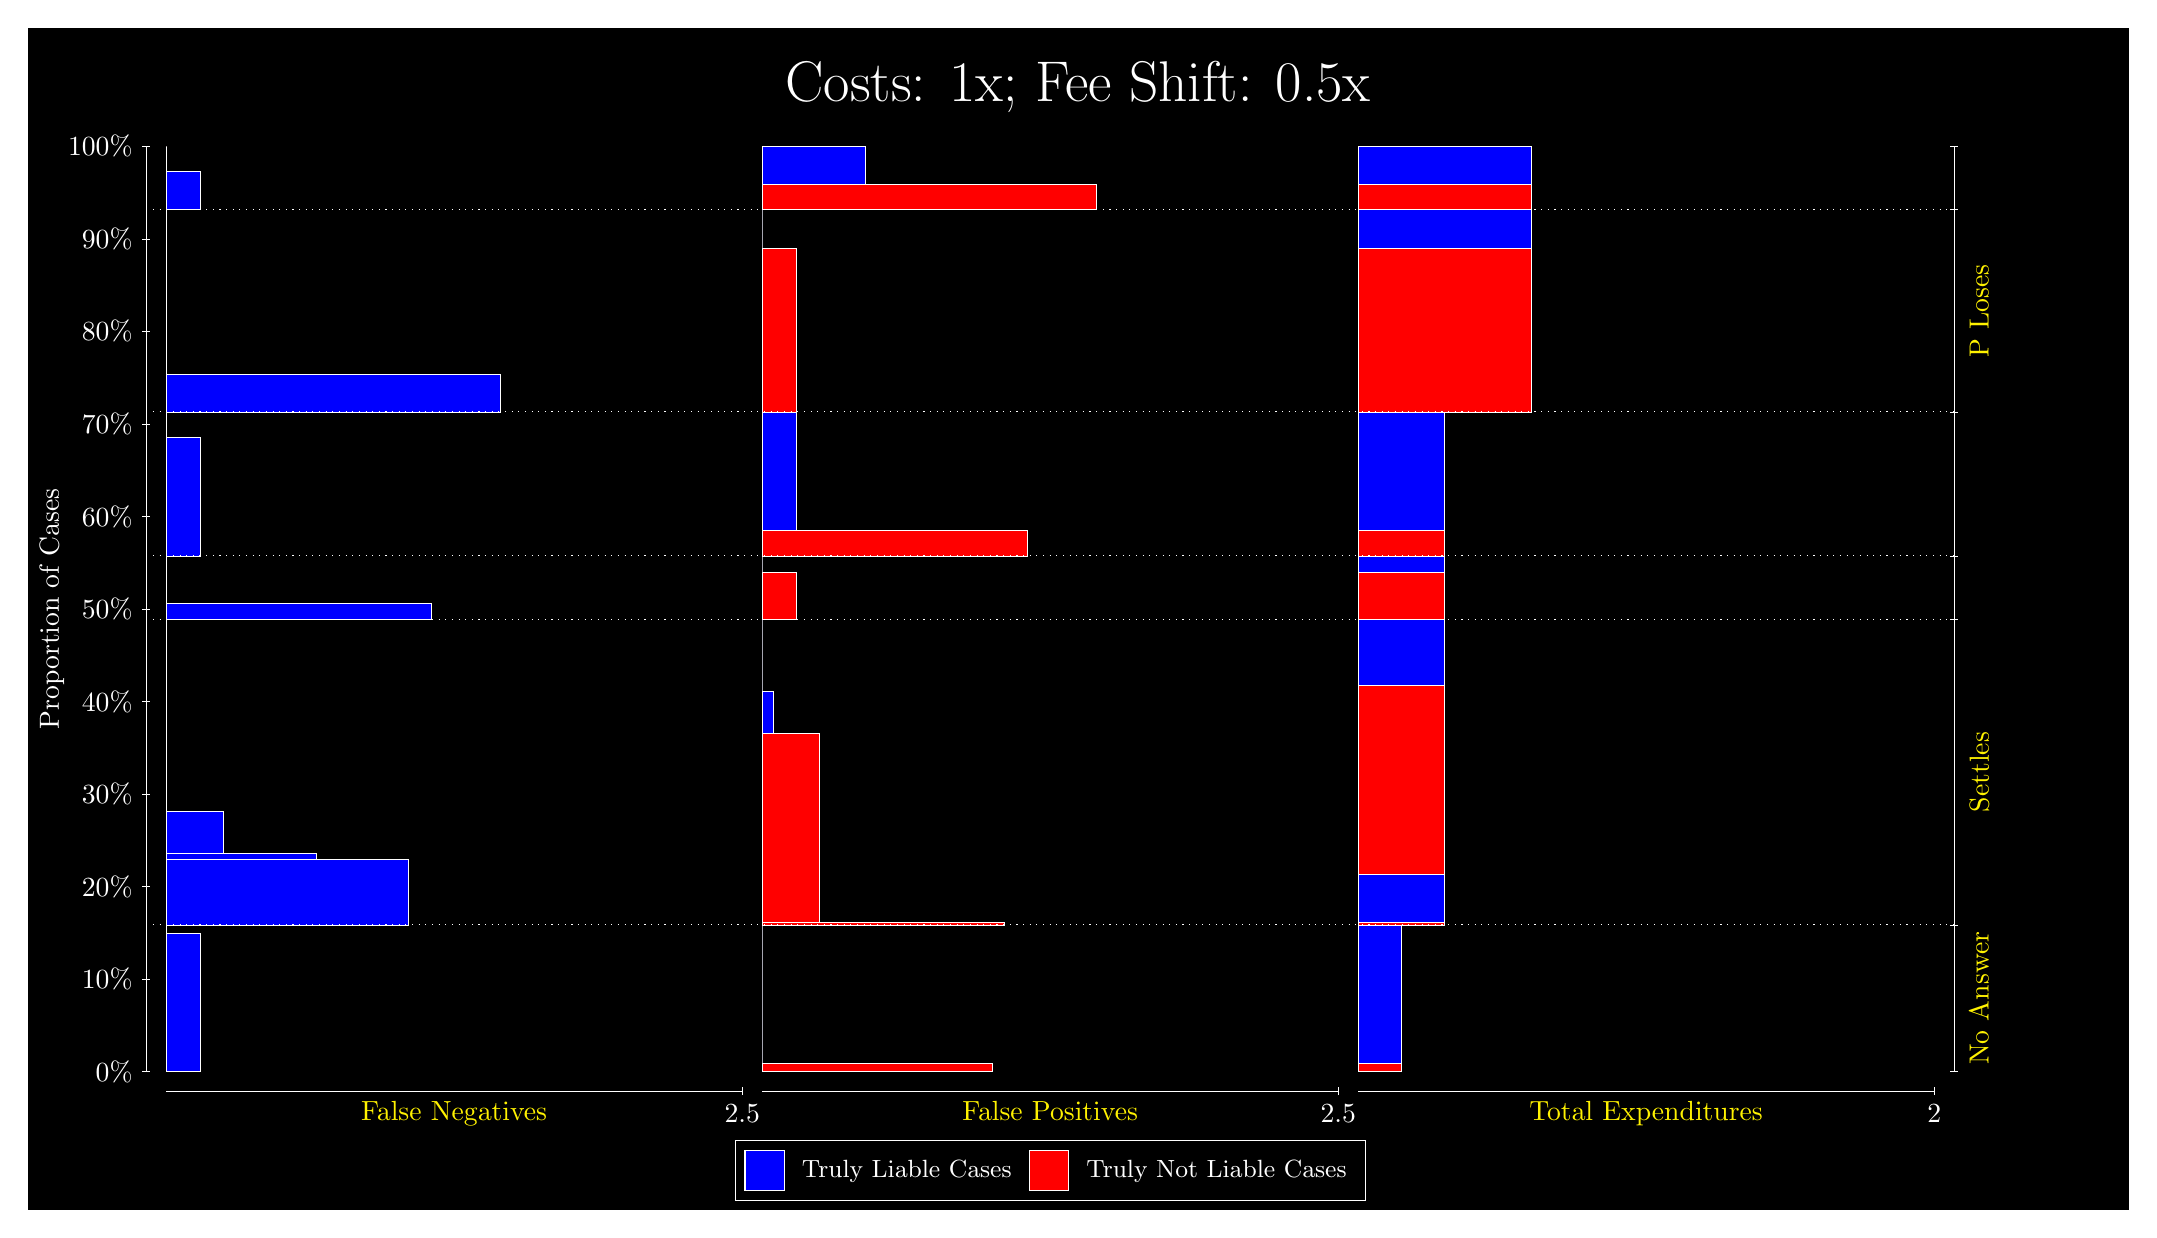
\begin{tikzpicture}
\draw[fill=black] (0,0) rectangle (26.667,15);
\draw[text=white] (0,13.5) rectangle (26.667,15) node[midway] {\huge Costs: 1x; Fee Shift: 0.5x};
\draw[white, very thin] (1.5,1.75) -- (1.5,13.5);
\node[rotate=90, text=white, anchor=center] at (0.3, 7.625) {Proportion of Cases};
\draw[white, very thin] (1.45,1.75) -- (1.55,1.75);
\node[text=white, anchor=east] at (1.45, 1.75) {0\%};
\draw[white, very thin] (1.45,2.925) -- (1.55,2.925);
\node[text=white, anchor=east] at (1.45, 2.925) {10\%};
\draw[white, very thin] (1.45,4.1) -- (1.55,4.1);
\node[text=white, anchor=east] at (1.45, 4.1) {20\%};
\draw[white, very thin] (1.45,5.275) -- (1.55,5.275);
\node[text=white, anchor=east] at (1.45, 5.275) {30\%};
\draw[white, very thin] (1.45,6.45) -- (1.55,6.45);
\node[text=white, anchor=east] at (1.45, 6.45) {40\%};
\draw[white, very thin] (1.45,7.625) -- (1.55,7.625);
\node[text=white, anchor=east] at (1.45, 7.625) {50\%};
\draw[white, very thin] (1.45,8.8) -- (1.55,8.8);
\node[text=white, anchor=east] at (1.45, 8.8) {60\%};
\draw[white, very thin] (1.45,9.975) -- (1.55,9.975);
\node[text=white, anchor=east] at (1.45, 9.975) {70\%};
\draw[white, very thin] (1.45,11.15) -- (1.55,11.15);
\node[text=white, anchor=east] at (1.45, 11.15) {80\%};
\draw[white, very thin] (1.45,12.325) -- (1.55,12.325);
\node[text=white, anchor=east] at (1.45, 12.325) {90\%};
\draw[white, very thin] (1.45,13.5) -- (1.55,13.5);
\node[text=white, anchor=east] at (1.45, 13.5) {100\%};

\draw[white, very thin] (24.457,1.75) -- (24.457,13.5);
\draw[white, very thin] (24.407,1.75) -- (24.507,1.75);
\node[anchor=west] at (24.407, 1.75) {};
\draw[white, very thin] (24.407,3.6116) -- (24.507,3.6116);
\node[anchor=west] at (24.407, 3.6116) {};
\draw[white, very thin] (24.407,7.4957) -- (24.507,7.4957);
\node[anchor=west] at (24.407, 7.4957) {};
\draw[white, very thin] (24.407,8.2995) -- (24.507,8.2995);
\node[anchor=west] at (24.407, 8.2995) {};
\draw[white, very thin] (24.407,10.127) -- (24.507,10.127);
\node[anchor=west] at (24.407, 10.127) {};
\draw[white, very thin] (24.407,12.696) -- (24.507,12.696);
\node[anchor=west] at (24.407, 12.696) {};
\draw[white, very thin] (24.407,13.5) -- (24.507,13.5);
\node[anchor=west] at (24.407, 13.5) {};

\draw[white, very thin, fill=blue] (1.75,1.75) rectangle (2.1891,3.5025);
\draw[white, very thin, fill=red] (1.75,3.5025) rectangle (1.75,3.6116);
\draw[white, very thin, fill=blue] (1.75,3.6116) rectangle (4.8239,4.4481);
\draw[white, very thin, fill=blue] (1.75,4.4481) rectangle (3.6529,4.5237);
\draw[white, very thin, fill=blue] (1.75,4.5237) rectangle (2.4819,5.0589);
\draw[white, very thin, fill=red] (1.75,5.0589) rectangle (1.75,7.4957);
\draw[white, very thin, fill=blue] (1.75,7.4957) rectangle (5.1167,7.7018);
\draw[white, very thin, fill=red] (1.75,7.7018) rectangle (1.75,8.2995);
\draw[white, very thin, fill=blue] (1.75,8.2995) rectangle (2.1891,9.803);
\draw[white, very thin, fill=red] (1.75,9.803) rectangle (1.75,10.127);
\draw[white, very thin, fill=blue] (1.75,10.127) rectangle (5.9949,10.611);
\draw[white, very thin, fill=red] (1.75,10.611) rectangle (1.75,12.696);
\draw[white, very thin, fill=blue] (1.75,12.696) rectangle (2.1891,13.177);
\draw[white, very thin, fill=red] (1.75,13.177) rectangle (1.75,13.5);
\draw[white, very thin, fill=red] (9.3189,1.75) rectangle (12.246,1.8591);
\draw[white, very thin, fill=blue] (9.3189,1.8591) rectangle (9.3189,3.6116);
\draw[white, very thin, fill=red] (9.3189,3.6116) rectangle (12.393,3.6441);
\draw[white, very thin, fill=red] (9.3189,3.6441) rectangle (11.222,3.6496);
\draw[white, very thin, fill=red] (9.3189,3.6496) rectangle (10.051,6.0484);
\draw[white, very thin, fill=blue] (9.3189,6.0484) rectangle (9.4652,6.5836);
\draw[white, very thin, fill=blue] (9.3189,6.5836) rectangle (9.3189,7.4957);
\draw[white, very thin, fill=red] (9.3189,7.4957) rectangle (9.758,8.0934);
\draw[white, very thin, fill=blue] (9.3189,8.0934) rectangle (9.3189,8.2995);
\draw[white, very thin, fill=red] (9.3189,8.2995) rectangle (12.686,8.6232);
\draw[white, very thin, fill=blue] (9.3189,8.6232) rectangle (9.758,10.127);
\draw[white, very thin, fill=red] (9.3189,10.127) rectangle (9.758,12.211);
\draw[white, very thin, fill=blue] (9.3189,12.211) rectangle (9.3189,12.696);
\draw[white, very thin, fill=red] (9.3189,12.696) rectangle (13.564,13.019);
\draw[white, very thin, fill=blue] (9.3189,13.019) rectangle (10.636,13.5);
\draw[white, very thin, fill=red] (16.888,1.75) rectangle (17.437,1.8591);
\draw[white, very thin, fill=blue] (16.888,1.8591) rectangle (17.437,3.6116);
\draw[white, very thin, fill=red] (16.888,3.6116) rectangle (17.986,3.6496);
\draw[white, very thin, fill=blue] (16.888,3.6496) rectangle (17.986,4.2605);
\draw[white, very thin, fill=red] (16.888,4.2605) rectangle (17.986,6.6592);
\draw[white, very thin, fill=blue] (16.888,6.6592) rectangle (17.986,7.4957);
\draw[white, very thin, fill=red] (16.888,7.4957) rectangle (17.986,8.0934);
\draw[white, very thin, fill=blue] (16.888,8.0934) rectangle (17.986,8.2995);
\draw[white, very thin, fill=red] (16.888,8.2995) rectangle (17.986,8.6232);
\draw[white, very thin, fill=blue] (16.888,8.6232) rectangle (17.986,10.127);
\draw[white, very thin, fill=red] (16.888,10.127) rectangle (19.083,12.211);
\draw[white, very thin, fill=blue] (16.888,12.211) rectangle (19.083,12.696);
\draw[white, very thin, fill=red] (16.888,12.696) rectangle (19.083,13.019);
\draw[white, very thin, fill=blue] (16.888,13.019) rectangle (19.083,13.5);
\draw[white, dotted] (1.5,3.6116) -- (24.457,3.6116);
\draw[white, dotted] (1.5,7.4957) -- (24.457,7.4957);
\draw[white, dotted] (1.5,8.2995) -- (24.457,8.2995);
\draw[white, dotted] (1.5,10.127) -- (24.457,10.127);
\draw[white, dotted] (1.5,12.696) -- (24.457,12.696);
\draw[white, very thin] (1.75,1.5) -- (9.0689,1.5);
\node[text=yellow, anchor=north] at (5.4094, 1.5) {False Negatives};
\draw[white, very thin] (9.0689,1.45) -- (9.0689,1.55);
\node[text=white, anchor=north] at (9.0689, 1.45) {2.5};

\draw[white, very thin] (9.3189,1.5) -- (16.638,1.5);
\node[text=yellow, anchor=north] at (12.978, 1.5) {False Positives};
\draw[white, very thin] (16.638,1.45) -- (16.638,1.55);
\node[text=white, anchor=north] at (16.638, 1.45) {2.5};

\draw[white, very thin] (16.888,1.5) -- (24.207,1.5);
\node[text=yellow, anchor=north] at (20.547, 1.5) {Total Expenditures};
\draw[white, very thin] (24.207,1.45) -- (24.207,1.55);
\node[text=white, anchor=north] at (24.207, 1.45) {2};

\node[text=yellow, centered, rotate=90] at (24.777, 2.6808) {No Answer};
\node[text=yellow, centered, rotate=90] at (24.777, 5.5537) {Settles};


\node[text=yellow, centered, rotate=90] at (24.777, 11.411) {P Loses};


\draw (12.978300999999998,1.5) node[draw=none] (baseCoordinate) {};
\begin{scope}[align=center]
        \matrix[scale=0.5, draw=white, below=0.5cm of baseCoordinate, nodes={draw}, column sep=0.1cm]{
            \node[rectangle, draw, minimum width=0.5cm, minimum height=0.5cm, fill=blue] {}; &
            \node[draw=none, font=\small, text=white] (B) {Truly Liable Cases}; &
            \node[rectangle, draw, minimum width=0.5cm, minimum height=0.5cm, fill=red] {}; &
            \node[draw=none, font=\small, text=white] (B) {Truly Not Liable Cases}; \\
            };
\end{scope}

\end{tikzpicture}
\end{document}